\documentclass[a4paper,12pt,twoside]{book}
\usepackage[utf8]{inputenc}
\usepackage[english]{babel}
%\usepackage{fontspec}
%\setmainfont[
%  Ligatures=TeX,
%  Extension=.otf,
%  BoldFont=cmunbx,
%  ItalicFont=cmunti,
%  BoldItalicFont=cmunbi,
%  SlantedFont=cmunsl
%]{cmunrm}

%\usepackage{polyglossia}
%\setmainlanguage{spanish}

\usepackage[c5paper]{geometry}
%\geometry{inner=2.5cm,outer=2.5cm,bmargin=3.2cm}
%\usepackage[DIV=14,BCOR=2mm,headinclude=true,footinclude=false]{typearea}

%\usepackage{ulem} %Hace que \emph sea subrayar

%\usepackage[p,osf]{scholax}
%% T1 and textcomp are loaded by package. Change that here, if you want
%% load sans and typewriter packages here, if needed

\usepackage{ebgaramond}
%\usepackage[type1]{libertine} % Linux Libertine for zweispaltige Texte
%\usepackage{textcomp}% Required to get special symbols
\usepackage[scaled=.8]{DejaVuSansMono}% FiraMono Typewriter font
\usepackage{PTSansNarrow} 
%\gilliuscondensed
%\usepackage[sfdefault]{FiraSans}
%\usepackage{bm}% Extra bold faces
%\usepackage[lf]{carlito}

\usepackage{lettrine} %Capital letters at the beginning of a chapter
\usepackage[activate={true,nocompatibility},final,tracking=true,kerning=true,spacing=true,factor=1100,stretch=10,shrink=10]{microtype}
\SetTracking{encoding={*}, shape=sc}{-20} % versalitas menos separadas
% activate={true,nocompatibility} - activate protrusion and expansion
% final - enable microtype; use "draft" to disable
% tracking=true, kerning=true, spacing=true - activate these techniques
% factor=1100 - add 10% to the protrusion amount (default is 1000)
% stretch=10, shrink=10 - reduce stretchability/shrinkability (default is 20/20)

%\usepackage{array,multirow,booktabs,colortbl,chngcntr} % El último es para counterwithout;
\usepackage[strict]{changepage}
%\usepackage{caption}
%\captionsetup{format=plain,labelsep=newline,labelfont={small,sc},
%textfont={small,it},singlelinecheck=false}
\usepackage[Bjornstrup]{fncychap} % Para cabeceras de capítulos sofisticados:     Sonny,    Lenny,    Glenn,    Conny,    Rejne,    and Bjarne.

\usepackage{graphicx,wrapfig,booktabs,multicol} % wallpaper: poner imágenes de fondo; wrapfigure: figuras a un lado del texto
%\graphicspath{{figures/}}
\usepackage{fancyhdr}
\usepackage{emptypage,pdfpages,fancybox} % Para que las páginas en blanco no tengan encabezado;
\usepackage{enumitem} %paralist: para compactenum, enumerate sin espacios
%\setlist[itemize]{nosep} %Espacio entre items en itemize
\usepackage[hyperref]{xcolor}
\usepackage[hidelinks]{hyperref}
\usepackage{xurl}

%\usepackage{minipage}

%\usepackage{quotchap} %Encabezados de capítulos
\usepackage{syntonly,verbatim}
%\syntaxonly

\usepackage{setspace,xspace} % xspace: Da \xspace para no tener que poner {} después de los comandos; pdflscape: páginas en horizontal;

\newenvironment{quotex}{\begin{quote}\small}{\end{quote}}
\newenvironment{quotationx}{\begin{quotation}\small}{\end{quotation}}


\begin{document}

% Por alguna razón, los marginados se creaban al revés. Así los corrijo. Feo, pero eficaz:
\let\tmp\oddsidemargin
\let\oddsidemargin\evensidemargin
\let\evensidemargin\tmp
\reversemarginpar

%\setcounter{secnumdepth}{4} % Para que llegue a numerar hasta las subsubsecciones;
%\renewcommand{\heavyrulewidth}{0.14em} % Grosor de las líneas extremas de las tablas;
%\renewcommand\thempfootnote{\alpha{mpfootnote}} % Símbolo de notas dentro de minipage
%\let\oldcaptionof\captionof
%\renewcommand{\captionof}[2]{\oldcaptionof{#1}{\newline \textit{#2} }}
%\renewcommand{\tablename}{Tabla}
%\counterwithout{figure}{chapter}
%\counterwithout{table}{chapter} % Así la numeración es 1, 2, 3... y no 1.1, 1.2... y no reinicia la num. en cada capítulo;

%\providecommand{\ggl}{\guillemotleft}
%\providecommand{\ggr}{\guillemotright\xspace}
\providecommand{\flright}[1]{\begin{flushright}#1\end{flushright}}
\providecommand{\flrightit}[1]{\begin{flushright}\itshape #1\end{flushright}}
%\renewcommand\UrlFont\sffamily
\urlstyle{tt}

\pagestyle{fancy}
\renewcommand{\sectionmark}[1]{\markright{#1}}
\renewcommand{\chaptermark}[1]{\markboth{#1}{}}

%Portada:
%\includepdf{00Portada}

\frontmatter
%
%\onehalfspacing
%\pagenumbering{Roman} %gobble es como empty

%\include{preindice}

%\fancyhf{}
%\fancyhead[LE]{\small \textbf{\thepage}$\quad$ Índice general}
%\fancyhead[RO]{\small Índice general $\quad$\textbf{\thepage}}
%\clearpage
\tableofcontents

%\doublespacing
\mainmatter

\fancyhf{}
\fancyhead[LE]{\small \thepage$\quad${\scshape\chaptername{} \thechapter}: \nouppercase{\itshape\leftmark}}
\fancyhead[RO]{\small \textsc{Section }\thesection{}: \nouppercase{\itshape\rightmark} $\quad$\upshape\thepage}
%\cfoot{\bfseries\thepage}

\pagenumbering{arabic}

%\onehalfspacing

% introductorios

\chapter{Introduction}
\section{Graduation Day}

Here are some suggested spiritual practices and how to know when success is achieved.

\paragraph{Detachment and Spiritual Combat}
The fundamental bases of our esoteric practice are detachment and spiritual combat. A sense of detachment needs to be developed. That is, you become the observer of your own life. You watch yourself make coffee, you watch yourself shave. Whenever you can, you wake up and observe.

In spiritual combat, you guard against the thoughts that enter your mind. You don't control what thoughts arise and when, but you do have some measure of control over what thoughts and images you allow to take root in your mind. If you are not diligent, then they can become obsessions, making it more difficult to root them out.

\paragraph{Intentional Suffering}
You must be willing to make sacrifices when necessary. The first thing to sacrifice is negativity. Yes, people love their negativity and are reluctant to give it up.

Suffering out of love is of a different character. If you give up your meal so your child does not go hungry, your pain turns to joy as you see his hunger satisfied.

Abstinence is the intentional denial of certain beneficial foods for a higher purpose. A common one is to give up meat. We see that in the story of Cain and Abel. Ask yourself what they had for dinner.

Cain had a loaf of bread, since that is all he had. Abel also ate a loaf of bread because he had sacrificed his meat earlier. That is why Abel's sacrifice was accepted; Cain didn't really sacrifice anything.

Purgatory is often misunderstood as a form of punishment. Rather it is a purification, because that process was neglected on earth. According to St. Catherine of Genoa, the souls in purgatory are happy because they know they are doing God's will.

\paragraph{The Persona and Conscious Acting}
The soul life contains many persona, which are the roles we play in our family and social lives. As such, they are necessary. However, there is a problem when the Ego starts identifying with one of those roles, or Persona. We need to be aware of the roles we play. Eventually, you can start playing them consciously and deliberately.

\paragraph{Collective Unconscious}
The task of individuation is achieved when there is harmony and equilibrium between the spontaneity of the unconscious and deliberate action by the conscious Ego. To maintain this equilibrium, unconscious processes compensate for the conscious ego to balance the psyche as a whole. These unconscious processes will correct for the egotistical bundle of personal wishes, fears, hopes, and ambitions. However, self-knowledge will ameliorate the effects of these processes, which manifest as irrational and uncontrollable impulses. As consciousness is widened, the actions of the ego will be freed from these unconscious corrections.

Clearing away the fog of this personal unconscious will reveal a deeper layer, called the collective unconscious. Man's mind is not a blank slate. Rather, the common heritage of the human race is contained in the mind as archetypes, which manifest themselves endlessly in history. Jung gives as examples the parent archetype, which is the reflection of the parent in the child. Of course, the collective imago is intertwined with a personal imago, since the child cannot fully understand the parent. There is also the imago of the child itself. This allows for the spontaneity of play. One can become child-like in this regard, which is not at all the same as being childish.

A man will have an interior image of a woman (anima) and a woman, that of a man (animus). The Sage is another one, since everyone tries to be wise to some extent in his own life. The human mind is prepared for psychic life just as the body is prepared for material life. It is inborn in him. Jung writes about it:

\begin{quotex}
The whole nature of man presupposes woman, both physically and spiritually. His system is tuned in to woman from the start, just as it is prepared for a quite definite world where there is water, light, air, salt, carbohydrates, etc. The form of the world into which he is born is already inborn in him as a virtual image. Likewise parents, wife, children, birth, and death are inborn in him as virtual images, psychic aptitudes. These a prior categories have by nature a collective character; they are images of parents, wife, and children in general, and are not individual predestinations. … They are in a sense the deposits of all our ancestral experiences, but they are not the experiences themselves. 

\end{quotex}
\paragraph{Psychology and Esoterism}
When Jung writes as a scientist, he must necessarily limit himself to the phenomena of psychic (i.e., psychological) events. Whether there is something beyond the phenomena is opaque to the scientific method.

On the other hand, the esoterist is definitely interested in what is beyond the merely psychic layer of life. Now Jung in his personal life did indeed believe in the reality of a noumenal reality beyond phenomena. Nevertheless, we are less interested in his spiritual writings, but his immense psychological knowledge can be used profitably.

\paragraph{Megalomania}
There are two main obstacles to spiritual development: the tendency to megalomania and sexual obsession. The former manifests as an unjustified high opinion of oneself. Jung write about several such cases. Such an individual will underrate, belittle, or criticize others, especially those close to him. He shows how unconscious processes will compensate for those feelings.

However, on our path, we don't rely on such unconscious processes. Rather, our method is deliberate and conscious. We notice that this megalomania manifests as “taking accounts”, that is, we are keeping track of all the alleged snubs and mistreatments we have received from others. By observing this tendency in a detached way, the Self will compensate consciously and we make find that such feelings simply dissipate.

It is necessary to “wake up” somehow in order to catch such manifestations “in the bud” as it were, before they can catch hold.

\paragraph{Song of Innocence}
It is accepted that childhood is a time of innocence free from overt, \emph{pace} Freud, sexual thoughts. This is followed by the time of experience. Once again, the notion that sexual activity in itself is somehow bad needs to be dispelled. Rather the issue is the misuse, or better said, the reuse of sexual energy. After the son of duty, different options present themselves. Like the faster, one can give up sex as a form of deliberate suffering, not because it is bad.

The goal is self-mastery, but it soon becomes clear that the desire is quite intense. It doesn't suffice not to engage in sex, because once the idea of it comes into the mind, it will recur, usually in an even stronger way. So it is really a spiritual rather than a material battle. It is a matter of guarding the thoughts.

Perhaps one can remain in the state of innocence for an hour, for a day, even for several days. One becomes a child again, spontaneous and innocent. You stop looking at women with that leering look; you know what that feels like.

Freud wrote of the state of polymorphous perversity, in which sexual energy is not confined to the genital region. The entire body can be on edge. Sometimes it can be difficult to even look at a pretty woman, because the body feels so intense; you may need to shield your eyes in that case.

Often, you just feel really good all day long.

\paragraph{Anima}
The imago of a woman in a man is called the Anima. Jung describes it:

\begin{quotex}
Woman, with her very dissimilar psychology, is and always has been a source of information about things for which a man has no eyes. She can be his inspiration; her intuitive capacity, often superior to man's, can give him timely warning, and her feeling, always directed towards the personal, can show him ways which his own less personally accented feeling would never have discovered. 

\end{quotex}
I want to focus on the esoteric teaching rather than the psychological, although they are compatible. Originally the human being was whole, but such as we are (speaking from a man's point of view), there is a gap in consciousness where the woman belongs. There is one, and only one, who fits perfectly. She may not be found, so there are others who fit less perfectly; some are closer than others.

The two who find each other are called Polar Beings. From an experiential point of view, it suddenly seems as though another person is sharing the same body. Her thoughts become mixed up with your own thoughts, her feelings are your feelings. Times of separation are an ache, times together a joy.

There are states beyond this one, provided certain tests of purity are met. I don't know those states personally, so I'll hold off for now.

\paragraph{Self}
The end result of individuation is the birth of a Self, or Real I, beyond the conscious Ego. The Self is not scientific because it can never be an object of thought. It is noumenal and beyond the psyche. It includes the Ego as well as all the unconscious processes. However, the Self integrates them all into a whole, eliminating the multiple independent little selves that seem to exist.

From the psychological point of view, Jung claims that the experience of the Self and the experience of God are the same.

St. Catherine of Genoa goes beyond that when she writes:

\begin{quotex}
My Being is God, not by some simple participation but by a true transformation of my Being. 

\end{quotex}
\paragraph{Graduation Day}
Quite some time ago, I had been participating in a group for a few years. I noticed the repetitive nature of it and no one seemed to be progressing. There were the same stammerings, the same excuses, the same struggles. One woman expressed the joy she felt communing with the squirrels in the morning.

I suspected most were lying, because my descriptions of the inner life were more vivid — and shocking — than theirs. I had assumed that the two group leaders were following some special program. I learned later that they were just winging it. Moreover, once you moved beyond their own limited frame of reference, they sounded lost. And there was no metaphysical teaching sustaining it.

Not that it wasn't helpful to me, just the opposite. One night I asked the group leader, “When do we graduate?” His response was simple, “Just graduate,” he replied. So I never went back after that.

You graduate when the burden becomes light, as St. Catherine described. You have achieved more self-awareness. You are liberating yourself from the lower forces that enthrall you with anxiety, despair, worry, uncertainty, obsessions. There is no need for any of that.



\flrightit{Posted on 2018-05-04 by Cologero }

\begin{center}* * *\end{center}

\begin{footnotesize}\begin{sffamily}



\texttt{Lyon on 2018-05-06 at 16:10 said: }

This was brilliant on many levels. Thank you! 

One question for you…

You mentioned Freud in your post. My surface-level take on him is that he is a charlatan of the highest order and that his ideas are deleterious. What is your general assessment of him? Apologies if your explicit views on Freud have already been covered in your writings. I am a rather recent visitor to this site.

And a comment…

The St, Catherine of Genoa quotes were profound and sublime. The insights in her quoted words, used judiciously in your post, I found both deeply rooted and uplifting. I never heard of her before visiting this site (…I recalled you mentioning her previously in a post, so at the time I did a quick internet search of her; I will go back to read up on her further).

Thanks again!


\hfill

\texttt{Dennis on 2018-05-08 at 15:12 said: }

My problem isn't getting to “graduation day”, but knowing where to begin the journey properly in the first place in order to even chart a path to “graduation day.” There are just so many books, resources (such as this blog – which itself would take forever to read and digest systematically from beginning to end), etc., that just knowing where to begin and how to separate the wheat from the chaff, so to speak, is daunting. I find myself often flitting from one book to the next, one thinker to the next, with no clear plan or goal, and in a rush of enthusiasms that soon fade, then I move on, hoping the next book or thinker will be the that changes everything for me…and on and on… Any ideas or recommendations from anyone on where and how best to begin?


\hfill

\texttt{F on 2018-05-10 at 09:29 said: }

With the right desire the Bhagavad Gita and Boehmes Way to Christ should be enough to get you started.


\hfill

\texttt{Sean on 2018-05-11 at 12:29 said: }

Not sure how to reply to someone but this is for Dennis.

Dont worry about reading the right books. Start with simple actions in your daily life. I'll give 5 I started with. 

1. Make your bed every day

2. Do some physical activity, a walk, a few push-ups, anything. No need to go to the gym if it feels daunting.

3. Quit all drugs/drinking save special occasions like wine at a wedding.

4. Sacrifice some sort of food. I started with processed carbs and made my way to all meat except wild caught fish. (still have difficulty with sugar)

5. Think positive thoughts about all you people you encounter. It's easy to judge that obese lady who buys nothing but Pepsi at Walmart but try and only let yourself think something positive about her. Even if you can't confirm it. Sometimes I'll think “I bet she's a really great aunt” or something.


\hfill

\texttt{lenamaria5 on 2018-05-15 at 19:36 said: }

@Dennis, Sean gave some good suggestions. I have also struggled with flitting from book to book. Perhaps that's a product of my (our?) generation's digital consumption habits and general lack of focus. It is much better to concentrate one's efforts on a single work or thinker for a longer period, aiming for depth and not breadth. Read meditatively, rather than just seeking information. Set a much longer timeline than you think you need for a work. If you've read through it before the time is up, you've read too quickly. Gornahoor has a post on Lectio Divina that's very good, if you're interested in Holy Scripture.


\end{sffamily}\end{footnotesize}

\section{Reaching your full Potential}

\begin{quotex}
Every Real Man has realized all the possibilities of the human condition, but each one has done so in a way which is typical of him alone, and which differentiates him from all other Real Men. If that were not the case, how could there be room, in our world, even for beings who have not achieved that level? \flright{\textsc{Rene Guenon} \textit{in letter to Evola}}

\end{quotex}

\begin{wrapfigure}{rt}{0.4\textwidth}
\centering
 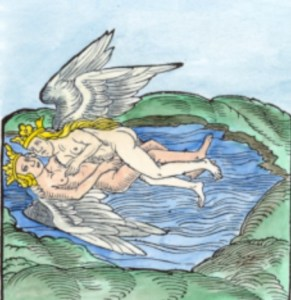
\includegraphics[scale=.4]{a20210321ReachingyourfullPotential-img001.jpg} 
\end{wrapfigure}

The first stage in esoteric teaching, the “Lesser Mysteries”, comprises everything related to the development of the possibilities of the human state. These possibilities transcend the activities of our ordinary life. The roles we play, such as family, occupation, and so on, are the fields of activity in which further development is made possible. Developing whatever talents we might have through education — the arts, science, sports, watching TV, and so on— may constitute the field of action that prepares us for higher possibilities, some obviously, better than others.

A fortiori, the search for powers or secret knowledge is fruitless, if not disadvantageous, from the esoteric perspective. These include:

\begin{itemize}
\item Fascination with vast conspiracy theories 
\item The search for psychic powers of all types 
\item The desire for mystical experiences 
\item Obsession with manifesting material objects 
\item Channeling higher beings 
\item Seeking secret knowledge of some sort 
\item Relying on psychedelics for spiritual experiences 
\end{itemize}
The common element is the focus on the corporeal and/or psychic worlds rather than the strictly spiritual part of oneself. \textbf{Rene Guenon} provides this admonition:

\begin{quotex}
[Psychic powers] are in fact a distraction in the rigorously etymological sense of the word. The one who lets himself be absorbed by the many activities of the corporeal world will never center his consciousness on higher realities, nor consequently develop within himself the corresponding possibilities. This will be all the more true for one who goes astray and disperses himself in the incomparably more vast and varied multiplicity of the psychic world, with its indefinite modalities. \flright{The “Rejection of Powers”, \emph{Perspectives on Initiation}}

\end{quotex}
This is not to deny the possibilities of such manifestations, which may arise as side-effects of mystical evolution. Nevertheless, our higher possibilities are not tied to any specific talents or abilities, since they are the principles which make those actions possible. From higher to lower, these are:

\begin{itemize}
\item True Will 
\item Consciousness 
\item Real I 
\end{itemize}
The attainment of these faculties completes the evolution of the possibilities of the human state, lifting the being to the Primordial State. Boris Mouravieff summarizes this succinctly:

\begin{quotex}
It is by this evolution that animal man can overcome Adam's Fall, can become a spiritual man, and so be initiated into divine wisdom. 

\end{quotex}
Then he is prepared for the Greater Mysteries.

\paragraph{Obstacles}
\begin{quotex}
Many are called but few are chosen. \flright{\textsc{Matthew 22:14}}

\end{quotex}
Here we encounter some immediate obstacles that prevent or discourage seekers.

\subparagraph{Unnecessary}
People believe that already have those faculties of a True Will, Consciousness, and a Real I. Hence, they don't see the need for esoteric training. They become more interested in phenomena.

\subparagraph{Explicit knowledge}
This type fails to understand the distinction between explicit and tacit knowledge. Explicit knowledge can be communicated through the written or spoken word. Tacit knowledge, on the other hand, cannot be communicated in that way. It is more like “knowing how” rather than in knowing. Tacit knowledge comes only by doing.

Like riding a bike or learning to swim, one has to actually do it. Reading a book about biking or swimming won't do it for you. Tacti knowledge is more effective if there is a guide, but most people are satisfied by reading or hearing theories about biking or swimming.

\subparagraph{Hard work}
\begin{quotex}
We can buy food for others; we can cook a dish with this food; we can serve it once it is cooked; we can cut it up; we can even act as if to put the food inside the mouth, as we do for a child or sick person. But at this point, each of us must make the necessary effort to swallow the food for ourselves; this cannot be done by anyone else. \flright{\emph{Gnosis I}}

\end{quotex}
Few people have the stamina or discipline to perform the exercises that transform explicit knowledge to tacit knowledge.

\subsubsection{Self-knowledge}
\begin{quotex}
When we close our eyes in an attempt to meditate, we are amazed to discover a boiler factory inside of us. \flright{\textsc{Joel Goldsmith}, \emph{The Art of Meditation}}

\end{quotex}
Meditation is sold today as an absolute good, that will relax us, lower blood pressure, and so on. However, if done properly, many, who believe that their inner life is nothing but Sunshine and Lollipops, are shocked to witness the “boiler factory” of irrelevant, fearful, or anxious thoughts that cast doubt rather than certainty.

It takes effort and persistence to get past that point.

\subparagraph{Inequality}
This teaching is the hardest to accept:

\begin{quotex}
Among several persons who receive an identical teaching, each one understands and assimilates it more or less completely and profoundly according to the range of his own intellectual possibilities, and in this way selection, without which there could be no genuine hierarchy, comes about quite naturally. \flright{\textsc{Rene Guenon}, \emph{Man and his Becoming according to the Vedanta}}

\end{quotex}
\paragraph{Higher Centers}
As mentioned in \textit{The Descent of the Absolute}\footnote{\url{https://www.gornahoor.net/?p=14019}}, the Emotional Center (animal soul) and Intellectual Center (intellectual soul) are divided into lower and higher centers. As we are born, the higher centers are undeveloped and are therefore only virtual. Esoteric training starts with the proper awakening or development of the higher centers.

Since our untrained emotional life is so erratic, mastery over the expression of the emotions is imperative in order to make further progress.

The Higher Emotional Center is located in the Heart, the seat of our Real I, the Sun center of our being. The Higher Intellectual Center is located at the level of the Head, the seat of consciousness.

\paragraph{Objective Art}
The first step in the in the development of the higher emotional center is to mitigate the effects of negative emotions. That opens up some space for more subtle emotions to manifest. Aids in the process include objective art, myths, and symbols. The focus of personal art is on the personality of the artist, while objective art is the reflection of higher ideas. The following passage refers to why, according to Plotinus, a sculpture is more beautiful than the block of stone from which it was carved.

\begin{quotex}
The real question is, why is the sculpted stone more beautiful? “The matter did not have this form, but it was in the one who thought, and before it came to the stone; but it was in the craftsman, not insofar as he had eyes or hands, but in that he shared in art” (Enneads V.8.1.16–19). If the sculpted stone is more beautiful than the lump, this is because thought, or idea, is more evident in it. The distinctive beauty of the sculpture, as opposed to the lump, is the form that it has received through the artist's work, which is an image of the form existing as pure thought-content, or idea, in the artist's mind. Consequently, the form, that is, the beauty, that renders the sculpture pleasing to behold is first and more truly in the artist's mind, as the paradigm of which the sculpture's beauty is an image. \flright{\textsc{Eric Perl}, \emph{Thinking Being}}

\end{quotex}
\paragraph{Myths and Symbols}
The purpose of Myths and Symbols is to reach these higher centers, the higher emotional and higher intellectual centers respectively. The attempt to understand myths and symbols by the lower mind will result in misinterpretation.

\paragraph{Sexual Sublimation}
Sexual energy can be redirected to the higher centers, which is the means to produce results.

\begin{quotex}
This consecration is produced by the sublimation of sex. Thus the circle closes itself. Each manifestation of life starts by a sexual act; at the end of the cycle, the activity of the sexual centre is manifested once more, but on a higher level, that of the higher centres, the level to which — by its nature — this centre belongs. \flright{\textit{Gnosis I}}

\end{quotex}
Ultimately, individual and group work will be replaced with Hieros gamos or polar couples. Since each one of the pair has a different way of knowing, their shared experiences enhance each other.

\begin{quotex}
The means … is to work as a couple. We must believe that in the new era which approaches, this method will be favoured more and more, will be protected, and will eventually become obligatory. However, for this esoteric work to be completed successfully by two people, it is essential that the two beings — man and woman — are integrally polar. 
\end{quotex}
\flrightit{Posted on 2021-03-21 by Cologero }

\begin{center}* * *\end{center}

\begin{footnotesize}\begin{sffamily}



\texttt{Greg on 2021-03-22 at 10:59 said: }

As to exercises does the form of Meditation matter? Is the Jesus prayer or say centering prayer effective in attaining these states or are other forms of exercises needed?


\hfill

\texttt{Tannheuser on 2021-03-22 at 12:47 said: }

I was actually just discussing this question of Objective vs. Personal art last night. 

I used the term “arbitrary” to describe what you call Personal art – to me it is boring because it does not participate in any universal idea or higher reality. That kind of art is usually a waste of time, because it doesn't offer any valuable possibilities to the one participating in it – just “A influences” imposing themselves and insisting on their own importance.

Interestingly, in contemporary art and entertainment, this arbitrary personal quality is the strongest in the so-called “high” arts (modern opera, painting, orchestral music, sculpture, architecture, and so on). Low or popular art often expresses less personal, more universal ideas, in the same way that folklore can preserve an echo the original spirit of a civilization long after the high art has become degenerate. Recently, however, there is a concerted effort to replace everything traditional even in low art with political propaganda (extending as far as 60 year old children's picture-books).


\hfill

\texttt{Arthur Konrad on 2021-03-23 at 09:20 said: }

@ Tannheuser,

Ever since the 19th century, opera and orchestral music is mostly an elaborate cacophony, operating on the same principle as a kid's toy made to produce some fabulous sound, after which the kid in question mutters `oooohhhh!' in awe – in other words, it is infantile. This is why Nietzsche loved Wagner, he had an infantile mentality. Most 19th century music was tailored to the tastes of women and effeminate men. Some operas of the romantic era are downright embarrassing. The bottom one and a half octave on the piano serves pretty much the same function. Most `virtuoso' pianists today play in a cacophonous way and abuse the bottom octaves as a rhythm section, and they think that a correct tempo does not exist. If you have healthy ears, you might as well shun piano performances for good, that thing is never going to get better.

Compare that nonsense to the masterpieces that are Baroque operas.


\hfill

\texttt{Paulo Adolpho on 2021-03-24 at 22:50 said: }

“A fortiori, the search for powers or secret knowledge is fruitless, if not disadvantageous, from the esoteric perspective. These include:

Fascination with vast conspiracy theories”

Cologero, why studying conspiracy theory, would it be negative? Don't you see that we must become aware, of who is trying to control and destroy this world, the anti-traditional forces?


\end{sffamily}\end{footnotesize}

\section{Rules too Difficult for Young Men}

The Internet has been able to create a new type of Star. The iSoapbox has given non-standard viewpoints a small space in which to be heard. There are the pretty right-wing girls who do well. However, men also gain larger audiences.

Recently a Star was born in the persona of a Canadian psychologist, and his influence has extended beyond the confines of the Internet. Part of his appeal, it has been said, is that he provides a positive message to young men. That may be true, even if the necessity for it is sad.

Once in a while, someone suggests to Cologero that he should be on TV. I'm sure they intend that as a sort of praise, although they have really not thought things through. First of all, the message here is a bit too difficult to summarize. The professor's worldview, on the other hand, can be summarized in a paragraph or perhaps in 12 rules for life. Then it is a matter of repetition.

Also — and I can say this — Cologero does not have a very dynamic personality. Not experiencing emotions like most of the world, he cannot imitate that pained, thoughtful look, nor does he weep on cue. Furthermore, he is quite low on “amiability”. He eschews current events and does not believe in “debates”.

Nevertheless, Gornahoor has touched on many of the same themes to a much smaller audience. These rules for life have been available online for several years with minimal impact. While Cologero is preoccupied, I've taken the liberty to propose Gornahoor's rules for life for young men. There must be some who can handle a deeper understanding of Life.

\paragraph{Stand up straight}
Those who have participated in the online seminars would have heard of the importance of posture since the very first meeting. Cologero has recommended the Alexander technique for those who still have trouble. Moreover, posture is just one aspect of a larger theme which includes voice, intonation, facial expression, and so on. Mastery of the body is part of self-development.

In a larger perspective, this includes physiognomy which includes more than just a face. Curiously, once out of favor, scientific interest in physiognomy has been growing.

\paragraph{Hierarchy}
\begin{quotex}
The authors of the Middle Ages could not imagine … the Universal Church without a pope. Because if the world is governed hierarchically, Christianity or the \emph{Sanctum Imperium} cannot be otherwise. Hierarchy is a pyramid which exists only when it is complete. \flright{\textsc{Valentin Tomberg}, \emph{Meditations on the Tarot}}

\end{quotex}
It is one thing to joke about the hierarchy of lobsters, but quite another to follow the hierarchy created by God. There is no need to repeat the details here, since the notion can be found throughout Gornahoor. There can be no compromise. It can be a difficult teaching because few want to accept voluntarily their rightful place in any hierarchy.

\begin{quotex}
A pyramid is not complete without its summit; hierarchy does not exist when it is incomplete. Without an Emperor, there will be, sooner or later, no more kings. When there are no kings, there will be, sooner or later, no more nobility. When there is no more nobility, there will be. Sooner or later, no more bourgeoisie or peasants. This is how one arrives at the dictatorship of the proletariat, the class hostile to the hierarchical principle, which latter, however, is the reflection of divine order. This is why the proletariat professes atheism. \flright{\textsc{Valentin Tomberg}, \emph{Meditations on the Tarot}}

\end{quotex}
\paragraph{Purification}
This is the metaphysical equivalent to “clean your room”. Granting that as a metaphor for “get you own life in order”, that is not possible without first getting your inner life in order. Here are some links to get you started.

\begin{itemize}
\item Purification of the Will\footnote{\url{https://www.gornahoor.net/?p=6950}}
\item Purity of the Mind\footnote{\url{https://www.gornahoor.net/?p=6961}}
\item Purification of the Word\footnote{\url{https://www.gornahoor.net/?p=6969}}
\item Purification of the Sex Act\footnote{\url{https://www.gornahoor.net/?p=6985}}
\item Purification of the Breath\footnote{\url{https://www.gornahoor.net/?p=6991}}
\item Moral purification of the Will\footnote{\url{https://www.meditationsonthetarot.com/moral-purification-of-the-will}}
\end{itemize}
\subsection*{Self-Mastery}
Self-mastery or autarchy is:

\begin{quotex}
For those who have absolutely possessed themselves, the alogon indicates only the unconditionality of his will, autarchy. Therefore, beyond the abstract intellectual, there is still an abyss between the man who lives his own life as lord and master, and the man who feels himself only as a demonic force of a nature that is passive to himself and that has its raison d'être outside himself. 

\end{quotex}
First, the autarch must master his thoughts, then his emotions, and ultimately his body insofar as it is possible. This is actually the Hermetic path, since each of those stages of self-mastery leads to the development of higher states of being.

\paragraph{Learn a martial art}
If so inclined, learn a martial art or become skilled in weaponry. A martial art develops concentration and attentiveness. The competition simulates life and death situations. Cologero wrote:

\begin{quotex}
A man, for his preparation, can conquer his fear of the elements: fire, air, water, and earth. Overcoming such fears leads to self-knowledge and a concentrated mind. Those with a warrior cast of mind need to excel at a martial art or develop skill with weaponry. Time spent in this way is more beneficial than excessive, or obsessive, reading. If you don't regard these activities as spiritual, then make them so. Do them with the right attitude and full consciousness. 

\end{quotex}
\paragraph{Spiritual Combat}
Spiritual combat is the analog of martial arts on a higher plane. However, at this level one's eternal life is at stake.

\begin{quotex}
Even without being killed a man can experience death, he can conquer, he can realize the culmination characteristic of a “super-life”. From a higher point of view, Paradise, the Kingdom of Heaven, Valhalla, the Island of the Heroes, etc., are only symbolic figurations forged for the masses, figurations that in reality designate transcendent states of consciousness, beyond life and death. The ancient Aryan tradition used the term \emph{jivan-mukti} to indicate such a realization while still in the mortal body. \flright{\textsc{Julius Evola}}

\end{quotex}
\paragraph{The Modern World}
It is necessary to have an adversary relationship to the modern world, even if only private. That means “to be in this world but not of it”. In anticipation of ridiculous comments, “modern” does not simply mean “contemporary”. We are neither Luddites nor Amish. Here are two of three steps (the third is in preparation).

\begin{itemize}
\item Understand the crisis of the Modern World 
\item Revolt against the Modern World 
\end{itemize}
\paragraph{Honor your father}
Honoring your father means gratitude for your inheritance and respect for those ancestors who created it. For Western Europeans, these are the three main currents of that inheritance.

\begin{itemize}
\item Hellenic Culture 
\item Roman Tradition 
\item Neoplatonic philosophy 
\end{itemize}
\textbf{Hellenic Culture}: The Hellenes have given us art, philosophy, political theory, and folk religion. Therefore, either create, or learn to appreciate, poetry, sculpture, drama (both tragedies and comedies). Develop a foundation in the trivium of grammar, logic, rhetoric: learn to speak well, logically, and persuasively. Learn the various types of political systems and the causes of their degeneration.

Pure thought is insufficient. A good life will include the Greek virtues: temperance, prudence, courage, and justice.

The Greek folk religion included reverence of ancestors, respect for the founders, and engaged the whole being in every aspect of life. Hegel describes it this way:

\begin{quotex}
In a folk religion in particular it is of the utmost importance that the imagination and the heart not be left unsatisfied: the imagination must be filled with large and pure images, and the heart roused to feelings of benevolence. 

\end{quotex}
\textbf{Roman Tradition}: The Romans brought us martial valor, administration, and engineering.

The primary Roman virtues included Piety, Gravitas, Dignitas, and either manliness or modesty.

\textbf{Neoplatonic Philosophy}: Neoplatonic philosophy integrated the best parts of Plato, Aristotle, and Stoicism. It is a powerful counterweight to contemporary philosophies of naturalism or materialism. A thinking man should always be an idealist, since the understanding of ideas is the aim of thought.

Start with \textbf{Augustine of Hippo}, \textbf{Dionysius the Areopagite}, and \textbf{Boethius}.

\paragraph{Conclusion}
If you've come this far, then draw your own conclusions.



\flrightit{Posted on 2018-03-17 by Aeneas }

\begin{center}* * *\end{center}

\begin{footnotesize}\begin{sffamily}



\texttt{manfred arcane on 2018-03-18 at 05:53 said: }

I see Peterson as a gateway drug, of sorts, to traditionalism. He is not there of course, not even close, but he is pointing people in the right direction and his lectures – if they bother to follow them – are providing them with tools with which they can approach a number of relevant thinkers. And, given his reach, that is a good thing – even if the 1\% of his followers decide to do a deep dive into Jung or Heidegger thanks to him, and even if the small portion of that 1\% eventually reaches the strain of thought that is espoused by the blogs like this one.


\hfill


\hfill

\texttt{Matt on 2018-03-19 at 08:44 said: }

George Heart, in his book “Christianity: Dogmatic Faith \& Gnostic Vivifying Knowledge” seeks to address the crisis of the lack of faith in modern people, by understanding the root cause, which is revealed in the Law of 3: the active force being the Church, the passive force being man's spirit/Personality, and the equilibrating force (the root of the issue) being change.

What has changed is that modern man has developed a stronger intellect, whereas the Church still preaches a simplistic “milk of the spirit” theology.

Perhaps this Canadian psychologist is gaining a foothold with many of his followers, on topics that don't usually have mass appeal (biblical analysis and hierarchy), partially due to his ability to engage and excite the intellect.

It's also interesting that he has discovered the hierarchical principle in nature, but fails to see it as the reflection of something higher.

http://matthewnanderson.wordpress.com/


\hfill

\texttt{LHOOQ on 2018-03-21 at 07:54 said: }

Manual of Epictetus is a good read to begin an ethical and philosophical life.


\hfill

\texttt{Kenneth Lyon MacNeil on 2018-03-25 at 14:33 said: }

A deep thank you to all who are responsible for the information and insights on this website. 

I will say little else till I do a deep dive into the information on offer here. I do look forward to doing so. 

Much appreciation,

\~{}Lyon


\hfill

\texttt{Robert on 2018-04-07 at 12:13 said: }

There are many traditionalist resonances in Peterson's work, as far as I can see, and he is far from being dismissive of religious belief. Quite the contrary. See, for example:

jordanbpeterson.com/philosophy/on-the-ark-of-the-covenant-the-cathedral-and-the-cross-easter-message-i/

Although I've seen no evidence that he has read Guénon, Schuon, Coomaraswamy or Evola, Eliade seems to have been important for him.


\hfill

\texttt{Bloom on 2021-03-18 at 17:59 said: }

Nice post, a lot of young men were captivated by Jordan Peterson for at least a year or two before moving onto greener pastures. He's a nice tutorial level boss.

Anyways, I want to add a comment on your last bit about the three main currents of Western Tradition. According to Evola, when we look at the Western Warrior Tradition, the three main currents are: Roman, Christian, and Nordic tradition.


\hfill


\end{sffamily}\end{footnotesize}


\section{Program for Beginners}

\begin{itemize}
\item Furnish your mind as completely as possible with the knowledge of how to inspect and control it. 
\item Train your body to obey your mind, and not to distract its attention. 
\item Control your mind to devote itself wholly to discover your True Will. 
\item Explore the course of that will till you reach its source, your Silent Self. 
\item Unite the conscious will with the True Will, and the conscious ego with the Silent Self. You must be utterly ruthless in discarding any atom of consciousness which is hostile or neutral 
\item Let this work freely from within, but heed not your environment, lest you make difference between one thing and another. Whatever it be, it is to be made one with you by love. 
\end{itemize}

\hfill

References

Crowley, Aleister. \textbf{The Law is for All}



\flrightit{Posted on 2010-09-28 by Aeneas }

\section{Scire, Potere, Audere, Tacere}

\begin{quotex}
\emph{Scire, Potere, Audere, Tacere}

To know, to be able, to dare, to keep silent

\flright{\textsc{Zoroaster}} 

\end{quotex}

\begin{wrapfigure}{rt}{0.35\textwidth}
\centering
 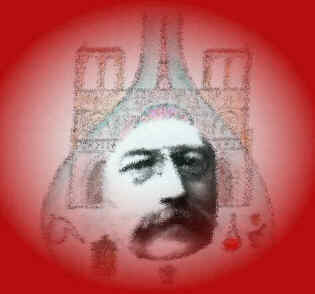
\includegraphics[scale=.25]{a20100928ScirePotereAudereTacere-img001.jpg} 
\end{wrapfigure}

Nature does not open the door of the sanctuary to anyone.

In these pages, the uninitiated will perhaps discover some proof of a genuine and positive science. I do not however, flatter myself that I shall convert them, for I know full well the obstinacy of prejudice and the great strength of preconceived opinions. The disciple will derive greater benefit form this book, provided always that he does not despise the works of the old Philosophers and that he studies with care and penetration the classical text, until he has acquired sufficient perception to understand the obscure points of the practice.

No one may aspire to possess the great secret, if he does not direct his life in accordance with the researches he has undertaken.

It is not enough to be studious, active, and persevering, if one has no firm principles, no solid basis, if immoderate enthusiasm blinds one to reason, if pride overrules judgment, if greed expands before the prospect of a golden future.

The mysterious science requires great precision, accuracy and perspicacity in observing the facts, a healthy, logical and reflective mind, a lively but not over-excitable imagination, a warm and pure heart. It also demands the greatest simplicity and complete indifference with regard to theories, systems and hypotheses, which are generally accepted without question on the testimony of books or the reputation of their authors, it requires its candidates to learn to think more with their own brains and less with those of others. Finally, it insists that they should check the truth of its principles, the knowledge of its doctrine and the practice of its operations from nature, the mother of us all.

By constant exercise of the faculties of observation and reasoning and by meditation, the novice will climb the steps leading to 

\paragraph{Knowledge}
A simple imitation of natural processes, skill combined with ingenuity, the insight born of long experience will secure for him

\paragraph{Power}
Having obtained that, he will still have need of patience, constancy and unshakeable will. Brave and resolute, he will be enabled by the certainty and confidence born of a strong faith, to

\paragraph{Dare}
Finally, when success has crowned so many years of labour, when his desires have been accomplished, the Wise Man, despising the vanities of the world, will draw near to the humble, the disinherited, to all those who work, suffer, struggle and weep here below. As an anonymous and dumb disciple of eternal Nature, he will remain faithful to his vow of silence. In Science, in Goodness, the adept must evermore

\paragraph{Keep Silent}

\flrightit{Posted on 2010-09-28 by Cologero }

\begin{center}* * *\end{center}

\begin{footnotesize}\begin{sffamily}



\texttt{Niko The Exile on 2019-02-15 at 00:18 said: }

This is exceptional, this so much reminds one of the Desert Fathers, i wonder if they were on the same wavelength as Fulcanelli.


\end{sffamily}\end{footnotesize}


\chapter{Spiritual exercises}
%Custodia de los pensamientos
\section{Mind Fasting}

In this time of year, many are making sacrifices such as giving up cupcakes or even añejo tequila. While there is a benefit to intentional suffering, it cannot happen in a mechanical way. Too often, it is thought of as the function of “will power”, that is the opposition of one desire (cupcakes) against another (sacrifice). What is really needed is to understand the relationship between personal effort and spiritual reality as we learn in the first Arcanum of Meditations on the Tarot. This is essential because 

\begin{quotex}
if one does not understand it (i.e. take hold of it in cognitive and actual practice), one would not know what to do with all the other Arcana.

\end{quotex}
Tomberg reveals the first and fundamental principle of esoterism:

\begin{quotex}
Learn at first concentration without effort; transform work into play; make every yoke that you have accepted easy and every burden that you carry light! 

\end{quotex}
This is also the key to Yoga as Pantajali tells us:

\begin{quotex}
Yoga is the suppression of the oscillations of the mental substance. 

\end{quotex}
These oscillations are automatic and mechanical: they arise from sensory impressions, inner desires, negative emotions, and thoughts that run on their own and usually have origins from unsuspected sources. Concentration is a free act and must be distinguished from obsession, which mimics concentration, but is not free.

\begin{wrapfigure}{rt}{.25\textwidth}
\centering
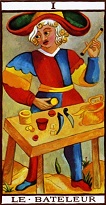
\includegraphics[scale=6]{a20121208MindFasting-img001.jpg}
\end{wrapfigure}

Intentional sacrifice then is training for concentration: we learn to distinguish the state of calm and freedom from the disorder of “desires, the imagination and discursive thought”. To be effortless, the will cannot oppose directly the sources of these disorders. Instead, we need to learn to detach from them, to observe them from a point of silence. Only then will they dissipate. This is the rational order of things, where the intellect is higher than, and dominates, thought and desire.

The season of Advent is the time of preparation for the incarnation of the Logos. Every physical event is the reflection of a spiritual reality and, since spiritual reality is timeless, it returns eternally. Hence, we can revisit the meditation on the second Arcanum as the Word is made Flesh.

There we see that the Logos is made incarnate by the Holy Spirit through the Holy Soul. As we are, the waters of our souls are full of perturbations. An event may create anger or anxiety, resulting in whirlpools that are hard to climb out from. There are tides coming in and out, so one day we say, believe, or vow one thing, and then the next day, just the opposite. Storms blow across the waters leaving them rough and choppy. In an unperturbed soul, the surface of the water is smooth line a pane of glass. Only in that condition will the Spirit be reflected clearly in the Soul. Otherwise, it gets mixed up with our fantasies and desires, which we too often take to be real expressions of the Spirit.

On the Feast of the Immaculate Conception we are reminded that only the Soul without sin can fully accept the Spirit. That Soul is totally free from perturbations. Can we even imagine what that is like? The exercise is worth the effort.

So either instead of, or in addition to, a physical fast, there is a Taoist exercise called mind fasting. If anyone has bothered to observe his thoughts, he will find abundant material to fast from. Perhaps there is a vulgar fantasy he indulges in. Perhaps he replays an event or conversations over and over in his mind. Perhaps he has a persistent anxiety or a worry. Maybe he has some daydream of success or power. Choose one and give it up. But give it up without effort.



\flrightit{Posted on 2012-12-08 by Cologero }

\begin{center}* * *\end{center}

\begin{footnotesize}\begin{sffamily}



\texttt{Senko on 2012-12-08 at 22:07 said: }

A most excellent post Cologero. Full of theory AND practical advice for one's everyday spiritual life. I find mental fasting much harder than physical fasting. I believe Advent is a most excellent time to prepare ourselves for the birth of Christ in our Heart. Blessings in Christ and Mary!\footnote{\url{http://senkosmos.blogspot.com.ar/}}


\hfill

\texttt{Mihai on 2012-12-09 at 14:43 said: }

Great post ! 

I would say that fasting has three different levels on which it must occur (like everything in the spiritual life, for that matter).

1. Physical: this is known by everyone and, unfortunetly, this is where it begins and ends in the mundane mentality of our age.

2. Psychic: just what you described here as “mind fasting”.

3. Spiritual: Without increasing prayer, meditation, study of Scripture etc. the whole thing collapses without purpose. 

I believe that when the fast turns into a petty legalism, limited to abstaining from certain foods and drinks, while ignoring the other two parts, it becomes even diabolical in character. I have seen a lot of people who do nothing but a physical fast and are most irritable and agressive during such a period.


\end{sffamily}\end{footnotesize}

%Oración
\section{Techniques of Prayer}

AÑADIR IMAGEN
With the initial disclaimer that (in the Christian religion) one must beware of “over-systematizing” the grace of God into specific techniques, the following is shared for the possible benefit of readers who are interested in esoteric Christianity.

Boris Mouravieff claims that there is a collection of “scripts” called the Golden Book in Orthodoxy, which is the oral tradition (or parallel to it, or a key, or fragments of it), which contain detailed teachings and instructions in the “secrets” of Christianity. I have been unable to locate references to it on the Internet, other than in Gnosis. This was the “teaching of Christ to the inner disciples”.

As I was reading \textit{Unseen Warfare} by Scupoli\footnote{\url{http://copiosa.org/spirituality/spiritual_combat.htm}}, a Venetian priest who had his book adopted into Orthodoxy and added to by \textbf{Theophan the Recluse}, I came across some advice to follow during prayer. Keep in mind that no prayer life will likely be effective without other ascetic practices (e.g., one can’t neglect fasting and expect prayer to come swiftly and easily). That said, and other advice followed (such as maintaining “a spirit of prayer” at all times), Theophan/Scupoli advise the following:

\begin{enumerate}
\item Pray in short prayers; these are lightning bolts which move swiftly to heaven, before the mental apparatus can intervene and subordinate the prayer to its own machinations.

\item Learn them by heart. This, contrary to popular belief, does the exact opposite of what opponents claim it does – it protects it from the vain repetitions of the discursive intellect, which stem from the gray matter, and not the body or the heart centers.

\item Focus attention on both the left nipple (the heart) and the throat chakra. This may seem odd, but perhaps some insight from Western alchemy\footnote{\url{http://hermetic.com/stavish/essays/lucid.html}} can help here (and others may have more to add from the East):

\end{enumerate}

\begin{quotex}
According to Sri Aurobindo, the throat center is associated with the externalization of mental forces, and the link between the higher and lower mental spheres. Like in some color scales of kabbalah, grey is associated with this center. In \textit{Serpent of Fire: A Modern View of Kundalini}, Darrel Irving points out that the \textit{Vissudha} chakra is presided over by the dual deities of \textit{Shakini} and \textit{Shiva}. Each is five faced, representing the five Elements, and three eyes, showing physical and psychic perception, or knowledge. Shakini is seen as Light itself, and Shiva, like the Hermetic ideal, is androgynous, half white and half gold. The center is associated with the purification of intelligence, the psychic substratum or ether (akasha), and hearing. The color given is smoky-purple. As with Sri Aurobindo’s color, purple is also sometimes given as associated with the throat center in modern kabbalistic works. Along with the remaining upper two psychic centers, these three constitute the only centers whereby \textit{direct psychic perception} is possible. In the West, the Throat center is less well defined, although it shares in all of the above named characteristics. In \textit{Kabbalah of the Golden Dawn}, Pat Zalewski states that the throat center is associated with the thyroid gland and controls respiration. As with yoga, each of the preceding centers is associated with an Elements, starting with Earth, Water, Fire, and Air. While not stated, it might be presumed that the Throat center is then the first center to be associated with Spirit, or Quintessence, as in yoga.
\end{quotex}

Since Christianity focuses upon “the Son” at the heart of the worlds, it is appropriate that the tradition of prayer associated with it would focus upon the two “linking chakras” between the lower and higher worlds. This is something Tomberg points out in Meditations.

Julian Lee, who is a “heretic” outside the Church, nonetheless has some very interesting considerations about prayer, Churches, and how Christianity is bhakti-yoga exotericized into a religion for the Western peoples.

\begin{quotex}
Why did my ancestors build their churches this way? Because men and women who think about God a lot get instincts about God’s nature. Thus my grandfathers and grandmothers of Europe designed their Sacred Places (churches) to evoke the thought of infinite space. They may not have done it consciously always, but they did it because they received instinctive knowledge of God through thinking of God. The White Europeans thought about the Transcendental Principle a great deal. They even had a special day reserved — every 7th day — for the thought of God alone. (What an amazing and cosmic-minded people our grandfathers and grandmothers were!) It was natural then that their churches evolved to evoke Akasa, one of the Creator-God’s first evolutes. Just as it was natural for them to build tall steeples representing the rectitude and straightness of the spine when aspiring for God, and the sublimated sexual energy made sacred by placing it in sacred limits (procreation and family), with the rest sublimated in aspiration for God.
\end{quotex}
 

And yet, the neo-pagan crowd in America (many of whom attend services each Sunday and talk a lot of God-talk) are trying to get away from the heritage of church bells, spires, folded or uplifted hands, and any kind of “weird” traditions in Christianity as fast as they can, desperately hoping to modernize and become up-to-date enough to slickly survive the end times. Even if Christianity survives what is coming, what will it look like?

I hope that some reading this can determine to hold onto the riches that God has already dumped in our laps, even at this late hour.

\flrightit{Posted on 2012-09-21 by Logres}

\chapter{Fasting}
\section{Mind Fasting}

In this time of year, many are making sacrifices such as giving up cupcakes or even añejo tequila. While there is a benefit to intentional suffering, it cannot happen in a mechanical way. Too often, it is thought of as the function of “will power”, that is the opposition of one desire (cupcakes) against another (sacrifice). What is really needed is to understand the relationship between personal effort and spiritual reality as we learn in the first Arcanum of Meditations on the Tarot. This is essential because 

\begin{quotex}
if one does not understand it (i.e. take hold of it in cognitive and actual practice), one would not know what to do with all the other Arcana.

\end{quotex}
Tomberg reveals the first and fundamental principle of esoterism:

\begin{quotex}
Learn at first concentration without effort; transform work into play; make every yoke that you have accepted easy and every burden that you carry light! 

\end{quotex}
This is also the key to Yoga as Pantajali tells us:

\begin{quotex}
Yoga is the suppression of the oscillations of the mental substance. 

\end{quotex}
These oscillations are automatic and mechanical: they arise from sensory impressions, inner desires, negative emotions, and thoughts that run on their own and usually have origins from unsuspected sources. Concentration is a free act and must be distinguished from obsession, which mimics concentration, but is not free.

\begin{wrapfigure}{rt}{.25\textwidth}
\centering
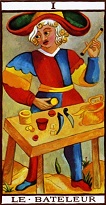
\includegraphics[scale=6]{a20121208MindFasting-img001.jpg}
\end{wrapfigure}

Intentional sacrifice then is training for concentration: we learn to distinguish the state of calm and freedom from the disorder of “desires, the imagination and discursive thought”. To be effortless, the will cannot oppose directly the sources of these disorders. Instead, we need to learn to detach from them, to observe them from a point of silence. Only then will they dissipate. This is the rational order of things, where the intellect is higher than, and dominates, thought and desire.

The season of Advent is the time of preparation for the incarnation of the Logos. Every physical event is the reflection of a spiritual reality and, since spiritual reality is timeless, it returns eternally. Hence, we can revisit the meditation on the second Arcanum as the Word is made Flesh.

There we see that the Logos is made incarnate by the Holy Spirit through the Holy Soul. As we are, the waters of our souls are full of perturbations. An event may create anger or anxiety, resulting in whirlpools that are hard to climb out from. There are tides coming in and out, so one day we say, believe, or vow one thing, and then the next day, just the opposite. Storms blow across the waters leaving them rough and choppy. In an unperturbed soul, the surface of the water is smooth line a pane of glass. Only in that condition will the Spirit be reflected clearly in the Soul. Otherwise, it gets mixed up with our fantasies and desires, which we too often take to be real expressions of the Spirit.

On the Feast of the Immaculate Conception we are reminded that only the Soul without sin can fully accept the Spirit. That Soul is totally free from perturbations. Can we even imagine what that is like? The exercise is worth the effort.

So either instead of, or in addition to, a physical fast, there is a Taoist exercise called mind fasting. If anyone has bothered to observe his thoughts, he will find abundant material to fast from. Perhaps there is a vulgar fantasy he indulges in. Perhaps he replays an event or conversations over and over in his mind. Perhaps he has a persistent anxiety or a worry. Maybe he has some daydream of success or power. Choose one and give it up. But give it up without effort.



\flrightit{Posted on 2012-12-08 by Cologero }

\begin{center}* * *\end{center}

\begin{footnotesize}\begin{sffamily}



\texttt{Senko on 2012-12-08 at 22:07 said: }

A most excellent post Cologero. Full of theory AND practical advice for one's everyday spiritual life. I find mental fasting much harder than physical fasting. I believe Advent is a most excellent time to prepare ourselves for the birth of Christ in our Heart. Blessings in Christ and Mary!\footnote{\url{http://senkosmos.blogspot.com.ar/}}


\hfill

\texttt{Mihai on 2012-12-09 at 14:43 said: }

Great post ! 

I would say that fasting has three different levels on which it must occur (like everything in the spiritual life, for that matter).

1. Physical: this is known by everyone and, unfortunetly, this is where it begins and ends in the mundane mentality of our age.

2. Psychic: just what you described here as “mind fasting”.

3. Spiritual: Without increasing prayer, meditation, study of Scripture etc. the whole thing collapses without purpose. 

I believe that when the fast turns into a petty legalism, limited to abstaining from certain foods and drinks, while ignoring the other two parts, it becomes even diabolical in character. I have seen a lot of people who do nothing but a physical fast and are most irritable and agressive during such a period.


\end{sffamily}\end{footnotesize}


\chapter{Memory}
\section{Immoral Dilemmas}

These are the results of my first experiments in remembering. Behind the temporal succession of the events of life, there is an eternal principle that gives them meaning and an intemporal I that is unchanged throughout.

The common view is that memory has something to do with the past, as when friends or family get together to relive their common nostalgic moments. Phenomenologically memory is bringing the past into the present. Or to put it another way, the seemingly disparate and unrelated events of life cannot be understood as merely temporal succession. As Rene Guenon expressed the goal in \emph{Oriental Metaphysics}:

\begin{quotex}
The person who attains this “primordial state” is still only a human individual and is without effective possession of any supra-individual states; he is nevertheless freed from time and the apparent succession of things is transformed for him into simultaneity. He consciously possesses a faculty which is unknown to the ordinary man and which one might call the “sense of eternity.” This is of extreme importance, for whoever is unable to leave the viewpoint of temporal succession and see everything in simultaneity is incapable of the least conception of the metaphysical order.

\end{quotex}
The exercise in remembering should lead to seeing one's life in its simultaneity. The events in their totality suddenly reveal a hidden meaning to life. This meaning is constant, eternal, and above time. What follows are some notes from this exercise. Keep in mind that there are four levels of memory of increasing depth:

\begin{enumerate}
\item \textbf{Intellectual memory}. The unadorned memory of a past event. 
\item \textbf{Emotional memory}. A memory that elicits an emotional reaction. 
\item \textbf{Volitional memory}. A memory that incites to action. 
\item \textbf{Moral memory}. A moral aspect is added to the memory. 
\end{enumerate}
Forgetting is analogous to death so remembering is life giving. Some memories arise spontaneously. Others take some effort. One should not stop at intellectual memory. It may take more effort to expand that memory to deeper levels. This essay has been some time in planning. The events mean nothing to you, but each time I've relived them, there is more intensity. Humor may be used to hide it. Nevertheless, over time, a common thread has been revealing itself to me.

You can avoid remembering now, but your entire life will be exposed at death. There is no point in evading the inevitable.



\flrightit{Posted on 2021-02-12 by Cologero }

\begin{center}* * *\end{center}

\begin{footnotesize}\begin{sffamily}



\texttt{Michael M on 2021-02-12 at 10:09 said: }

When it comes to viewing memories and the addition of the moral element and a common thread throughout life, the more we untangle those knots looking back and going further and further long those lines does give a different type of perspective or Gestalt of the whole. 

Utilizing that theme, would it be more advisable then to look at present / future events in the light of such a theme? Or is that too close to trying to get a specific result from a type of effort? Thereby destroying the whole effort to begin with. The building of a foundational “center” with a common theme that has always been present in life would reasonably seem to be the only true way to have a viewpoint or post for life that would never be carried away by external influences.


\hfill

\texttt{Tannheuser on 2021-02-12 at 13:24 said: }

““Say it, say it, say it.” Now I knew perfectly well what she wanted me to say, but I just couldn't say it. I was her one and only love but she was just one of many to me.

Tant pis pour elle. How much pain has unrestrained desire caused in the world? And why does it have to feel so good?”

—–

The girl who I couldn't “say it” to was actually the first woman I had ever slept with, and the most beautiful. Our relationship had started because I wanted to make the woman who I really loved at that time jealous, which worked. Still, for a while she sucked me into a world of immense pleasure that was hard to step away from. She had a very pleasing personality and the sex was incredible, but the whole thing was spiritually suffocating – I felt like Odysseus on Circe's island. 

In the end I only ever said “I love you” to three women, who corresponded in order to the types of ame-soeur, mistress, and wife.

—–

Michael M: If your life is a unity, then it only makes sense that you take action in the present from that perspective as you become conscious of your own meaning and purpose.


\end{sffamily}\end{footnotesize}

\section{Birth of the “I”}

In \emph{The I Problem and Genius}\footnote{\url{https://www.gornahoor.net/?page_id=12944}}, Weininger writes about the realization of the sense of the “I”, that is, the experience of being an independent centre of awareness. He proceeds to give examples (from Jean Paul, Novalis, and Schelling) where they describe their earliest experiences “of the possession of an ego in the highest sense.”

Some men seem to have had a strong experience of that, often from an early age, while others don't even seem to understand the question. Readers may want to consider this an exercise in self-realization and try to remember their own such experiences. Here are two of mine:

\begin{quotex}
The first shocking memory I recall is when I had just finished a BM. I opened the bathroom door and called to my mother to take a look at it in the bowl. I was dumbfounded when she did not want to look at it and told me to go flush it myself. At that moment I woke up to myself and realized I was on my own.

\end{quotex}
That had to have been around two and a half years old. The following one was probably a year later:

\begin{quotex}
I tied all my toy trucks and cars together and made a train. As I pulled it around the house, my sister was crawling behind the train and following it. This is my first recollection of the sense of having a “will”.

\end{quotex}


\flrightit{Posted on 2008-07-06 by Cologero }

\section{Thanks for the Memories}

\begin{quotex}
you must know, Sancho, if you do not know it already, that with lovers, the external actions and movements, revealed when the topic of their love arises, are reliable messengers bringing the news of what transpires deep in their souls. \flright{\textit{Don Quixote}}

\end{quotex}
Memory is not mere reminiscing, but is a progress from the past to the present. In Bergson's diagram, the base AB of the inverted cone is the memory. The Self S lives and acts on the plane P, bearing the weight of the past. If you forget your past, you will be driven by unconscious forces. Memory is real and actual only in the present, to the extent that it shapes our perception and understanding of the world.

Plato famously claimed that knowing is remembering. In particular, we have forgotten the world of essences, that is, the ideas in the mind of God; Hence, knowing an essence is just a recall of that which was forgotten. A fortiori, knowledge of the Self, our essence, and our destiny must also be a form of remembering. But memory of the forms takes place in stages. We understand more as we rise up through the states of being. Boris Mouravieff explains:

\begin{quotex}
\emph{Memory} is a direct function of the \emph{being} of the individual. The higher the level of \emph{being}, the better the memory and the greater its capacity to contain. Loss of memory, which causes the notion of the name and the ensemble that is attached to it to be forgotten, makes a madman out of a normal man: the sense of continuity is no longer present. 

\end{quotex}

\begin{wrapfigure}{rt}{.25\textwidth}
\centering
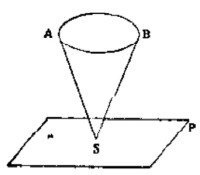
\includegraphics[scale=.5]{a20210131ThanksfortheMemories-img001.jpg} 
\caption{Memory Cone}
\end{wrapfigure}

The esoteric teaching is that forgetting is analogous to sleeping and to death, as they manifest on different levels. Valentin Tomberg makes it clear:

\begin{quotex}
For our whole experience (outer and inner) forgetting, sleep and death are three manifestations of the same thing —namely the “thing” which effects disappearance. It is said that sleep is the younger brother of death. It is necessary to add: forgetting is the brother of sleep. … One forgets, one goes to sleep, and one dies. One remembers, one awakes, and one is born. Remembering is to forgetting as awakening is to falling asleep, and awakening is to sleeping as birth is to death. … Natural forgetting reduces man to animality; natural sleep reduces him to vegetality; and natural death reduces him to minerality. 

\flright{\textit{Letter XIII, Death}}

\end{quotex}

Yet remembering is not simply bringing an image of the past into the present, since there are levels of depth to memory. You can remember solely with the intellect, with feelings, or even with the will. The highest is moral memory, based on love and all that accompanies it. Tomberg emphasizes the importance of the latter:

\begin{quotex}
It is love which is at work in moral memory when it recalls things from the past. Here it is admiration, respect, friendship, gratitude, affection and a thousand other things which have deeply moved you, which render things from the past unforgettable, i.e., evocable at each instant. The more one has loved, the more one remembers through moral memory.

Moral memory — which can comprehend everything without exception — is all the more effective the less one is morally indifferent. Indifference, a lack of moral interest, is the fundamental cause of the lapse of memory which often takes place in old age. The less one is indifferent, the more one remembers of the past and the more one is capable of learning new things. 

\end{quotex}
\paragraph{Moral Memory}
Moral memory predominates in old age. The young depend on mechanical memories, which arise spontaneously; this faculty becomes feebler with age. Hence, it must be replaced with intellectual or logical memory. This requires an active effort to remember things. People who neglected to learn how to make intellectual efforts in their youth, will become forgetful as they age. Tomberg goes even further, explaining that moral efforts are likewise necessary:

\begin{quotex}
People who are able to and who know how to give everything a moral worth and to see a moral sense in everything will not forget anything: they will have a normal, if not excellent, memory to a very advanced age.

Moral memory — which can comprehend everything without exception — is all the more effective the less one is morally indifferent. Indifference, a lack of moral interest, is the fundamental cause of the lapse of memory which often takes place in old age. The less one is indifferent, the more one remembers of the past and the more one is capable of learning new things. 

\end{quotex}
\paragraph{Love and Work}
\begin{quotex}
Love and work are the cornerstones of our humanness. \flright{\textsc{Sigmund Freud}}

\end{quotex}
To begin the experiment of “remembering”, one must first decide what to remember. If love and work are the cornerstones of our humanness, that is the place to start. When one loves, one cannot be morally indifferent. And our acts — our work, our projects, our adventures — only have significance when they are moral acts. So we turn to our favorite Knight Errant, Don Quixote, who had expertise in both realms, as a model.

Love was constantly on his mind, especially for the one special lady, who was the driving force, the creative force, for his life. He treated women with chivalry. Against men, he was prepared to do battle against iniquity and to protect the weak and helpless. He brandished his cold weapons to make a point. He did not carry around a copy of the constitution nor did he propose to reason with his enemies to make his point. That is why his deeds have been recorded and are remembered.

\paragraph{Pointillism}
Most people live their lives as an accumulation of points, one after the other. Events in their lives are unrelated to each other since points are unrelated. They are stuck in time and not in simultaneity. If you desire to live your life as a work of art, whom would you commission to paint it for you?

The realist will plan it in advance: he will make a detailed drawing, calculate the perspectives, choose the colours, lighting, etc. The end result is known even before the artist begins. The unsophisticated viewer prefers realism because it requires little or no effort from him.

The better choice is pointillism. As you live your life day to day, it is difficult to grasp it as a whole. Instead, your life appears to you as a series of points of various colours, almost at random, and it may not make sense as a whole at any given time. However, as the points are painted at various spots on the canvas, gradually the full image of your life can be discerned. But this takes more effort — and patience — by the viewer to wait for the points to begin to make sense.

So that is how to start, each memory is a point or set of related points. Over time, as they appear on the canvas of your life, the whole picture of your life should come into view.

\paragraph{Life is Short}
They say that life is too short. Your memories should be relevant; they should be predominantly moral memories. If your fondest memories are watching TV or hanging out at the pub, then your life is actually too long and you are trying to fill it up with trivialities.

To develop a moral memory, you must live by principles and your acts must have a point. This should be obvious, for the alternative is live a life that is unprincipled and pointless.

\paragraph{Dislikes, Fears, and Accidents}
The first step in deep remembering is to ascertain one's earliest likes, talents, and proclivities. This exercise is preferable to most people because it seems pleasant. However, one can gain more self-knowledge by remembering the things you did not like. What events transpired in your life that you did not desire? Can you see what role, however subtle, you may have played in bringing it about?

This applies also to what you most fear. How has the avoidance of this fear shaped your life?

Another consideration is to remember everything that occurred, seemingly by chance or accident. From the human point of view, that may seem to be the case. But can you dig even deeper to see if there is a state of being from which you willed those events.

Meditations like these will often bear great fruit.

\paragraph{Encounters with Others}
Your life is a world line in the cosmos. And everyone else has his own world line. Mathematically understood, a Point is where two Lines intersect. In other words, the points don't define the line, but the line defines the points that constitute it.

So when I see a Point, I don't ask what it means in isolation. Instead, I look for the two lines. Of course, you are one of them, and the other is a person you encounter. Why are two distinctly different world lines meeting at that point? From that perspective, you can experience the event in its wholeness, all at once, simultaneously.

There are natural reasons, of course, for the intersection of lines: family, jobs, food, love, revenge, and so on, i.e., all the things involved in human life. But that does not exhaust all the possibilities.

Nevertheless, some lines meet for no human purpose at all, yet you can't dismiss it as pointless because the Point is there and is unavoidable. You may choose to look away. That is possible because it is so ethereal. But that decision has its danger, since you may miss one of the most important moments in your life.

How many of those life events have you forgotten? and you may even be glad they are forgotten. How few of those memories will endure through eternity? It is imperative to know what to forget and what to remember.

Why have some people made an impact on your life and others not so much?

\paragraph{Things forgotten}
You will find memories best left forgotten. Something that had seemed so important and so impactful at that time, appears now in retrospect to be so distant, so far from your current level of being, that it may as well have been the memory of a different person. It may remain as an intellectual memory, but it no longer has any emotional impact, and it most certainly does not induce you to act.



\flrightit{Posted on 2021-01-31 by Cologero }

\begin{center}* * *\end{center}

\begin{footnotesize}\begin{sffamily}



\texttt{Michael M on 2021-01-31 at 10:26 said: }

“They say that life is too short. Your memories should be relevant; they should be predominantly moral memories. If your fondest memories are watching TV or hanging out at the pub, then your life is actually too long and you are trying to fill it up with trivialities.

To develop a moral memory, you must live by principles and your acts must have a point. This should be obvious, for the alternative is live a life that is unprincipled and pointless.”

You describe exactly my experience lately when I hear someone say “killing time”. Internally I watch my cage intensely when I see it in others and am watchful for it in my own domain. Quite insidious a phrase especially when understanding time as part of the compound nature of experience, life, and the unfolding of ideas. Don't want to fall asleep in a dream and dream our life away…

Has anyone found it more difficult at times to remember “facts” (academic / intellectual) memories when focusing on moral memory intensely? Or perhaps there is some type of learning curve or displacement of useless knowledge for rewriting of moral orientation?


\end{sffamily}\end{footnotesize}

\section{Immaterial Intimacy and Material Catastrophes}

\paragraph{Introduction by Cologero}

\begin{quotex}
and directing his gaze from now, on towards beauty as a whole, he should turn to the great ocean of beauty, and in contemplation of it give birth to many beautiful and magnificent speeches and thoughts in the abundance of philosophy. \flright{\textit{Diotima to Socrates in Plato's Symposium}}

\end{quotex}
Diotima was a prophetess and philosopher. In the Symposium, she explains the ladder of love, which comprises the following stages.

\begin{enumerate}
\item In youth one Is attracted to the physical beauty of the other. 
\item At this stage, the spiritual beauty of another person is more important. Therefore, love is now directed towards this person because of her moral, intellectual, and spiritual qualities. 
\item The beauty of knowledge itself becomes the focus. This is the love of Wisdom, or philosophy. 
\item Ultimately, one reaches the appreciation of Beauty apart from any individual, to consideration of Divinity, the source of Beauty, to love of Divinity. 
\end{enumerate}
If Diotima is speaking as a philosopher, those stages make sense. But not if she is speaking as a prophetess of the future since precious few manage to get beyond the first stage. However, in the timeless realm, the notions of past, present, and future are relative. In the Future of Prophecy, Saint Gregory the Great\footnote{\url{https://www.meditationsonthetarot.com/the-future-of-prophecy}} explains the three tenses of prophecy: future, present, past:

\begin{quotex}
prophecy is not a matter of prediction, but rather of revelation. That is why there can be a prophecy of the past and the present; prophecy uncovers hidden truths, truths concealed by time or by present circumstances. He writes: “Prophecy is present when something is concealed, not by the spirit, but by the absent Word, which however is laid bare by the Spirit.” 

\end{quotex}
Sibylle has done her own experiment in making the past present, through the act of remembering. She had been working on those memories for a long time and until recently never figured out what to make of them. Suddenly, their meaning was revealed to her. That is how she became Sibylle.

You can find her experience in the New Decameron at Immaterial Intimacy and Material Catastrophes\footnote{\url{https://gornahoor.net/decameron/immaterial-intimacy-and-material-catastrophes/}}.

As you try your own experiment, notice the extent that you have contributed to the events of your life, whether out of ignorance, by accident, or deliberately.


\hfill

\paragraph{The Chewing Gum Boy}

She really didn't like the boys in Kindergarten. They constantly bullied her, said mean words, started laughing in her presence. There was one boy especially cruel, quite obscene for a five-year-old. Very blonde, strong and he kept singing Nena's “99 Luftballons” using a huge wooden building brick as a microphone. One day when she went to the supermarket with her mother, they encountered this boy with his mother. The two mothers started talking and he was too embarrassed to look at her. She didn't care because she thought she didn't like him. All of a sudden, the boy reached out and handed her a chewing gum. When he finally looked at her, she knew that cruel boys would never pose a danger to her. They revealed their true feelings by their first glance.

\begin{wrapfigure}{rt}{.3\textwidth}
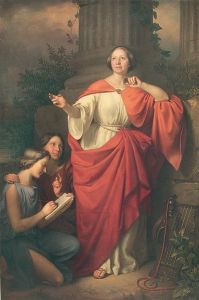
\includegraphics[scale=.5]{a20210215ImmaterialIntimacy-img001.jpg} 
\caption{Diotima}
\end{wrapfigure}

\paragraph{Ending up in the Boys Corner}
On her first day of elementary school, the girls of her class promised each other to stick together in order to avoid sitting next to a boy. When the teacher announced everybody should choose a seat, her best friend ran away to sit with another girl. So she picked a nice window seat next to a long-haired, fair looking girl. Suddenly the girls started laughing at her. When she looked around, she realised she was surrounded by boys. The fair looking girl turned out to be a boy — she spent the rest of the schoolyear by his side, but never figured out what he was either thinking or feeling. He remained completely alien to her.

\paragraph{The Teacher}
When she was thirteen, she switched violin teachers. Her father had taught her since she was four and made his daughter the winner of a several local music competitions. Now that she was supposed to win the national youth competition the stakes were high. A new coach was needed: a motivating, inspiring presence who would make her leap to the next level. The Teacher was indeed motivating and inspiring — mainly because she was terribly in love with him. She would have lessons at his home, eat lunch with his parents — he only touched her slightly, she told me that it felt like a breeze on her neck and arms. So she won the competition, everyone was happy except for her. Why? The Teacher was a decent man: winning was nice — but she wanted Love.

\paragraph{Love gone unnoticed}
After she dropped out of High School when she was 17 to advance her career, she went on a concert tour in the Czech Republic with two very sweet boys, a cellist and a pianist. They were part of a group of prizewinners of an international music competition playing concerts in Prague and Bohemia. She fell in love with the pianist, spent her evenings kissing him and enjoyed herself until one morning she discovered the ashes of a letter on the doorsteps of her motel room. She had no clue what that was all about. It turned out that the cellist had fallen in love with her, planned to open up to her in a love letter, but found out about her and the pianist. She hadn't noticed anything. She didn't feel sorry for him then. Maybe she does now.

\paragraph{The Tragedy of Napoli and Thanksgiving in Chicago}
During her first year at Indiana University, she met the Italian. He started calling her by his own last name as if they were already married. In fact they had barely exchanged a kiss. During the summer she went to visit him in Naples. Her parents had rented a house near Pisa for the holiday season and she took the train down to the South. She felt confident, had learned Italian in six weeks and was looking forward to meeting her future husband again. He was very passionate upon her arrival, but fell short of making love to her. Instead he called his best friend, a manic-depressive art student from Bloomington, who was spending his summer travelling around Italy. For the rest of her stay she spent more time with that best friend than with her supposed future husband. Back in Bloomington she kept hearing stories about him — that he had broken so many hearts, sleeping with every girl in town. Just not with her.

On Thanksgiving Day she decided to change the Matrix. Instead of letting things happen to her she allowed a student from Venezuela to take her virginity in a motel room in Chicago. He got mad at her for not telling him that it was her first time. She had simply assumed he wouldn't care and was stunned that he felt responsible for what she had made him do. Her first encounter with wrongly guided willfulness.

\paragraph{Mr. Nice Guy}
She did not love him at first. But she thought it was time to settle with a “nice” guy and found a seemingly willing partner in a German cellist she studied with in Amsterdam. They came from the same prude-protestant background and did everything right. Meeting both parents, spending time with his ersatz father — a highly skilled psychologist who kept emphasising how good she was for him after his ill-fated relationship with his former girlfriend. Still: he loved his ex-girlfriend and no other woman could make him happy. A couple of years ago the nice guy's ex-girlfriend committed suicide.

\paragraph{Another Change to the Matrix}
She tried another change to the Matrix. She felt trapped and pushed by external expectations and wanted to be left alone. So fifteen years ago she went online, picked herself a husband from a dating site, became pregnant and got married. Her husband was her best friend for a while. But he always seemed emotionally detached. When she finally managed to catch a glimpse of his Anima, she got scared. He was totally unaware of her. Everything she actively achieved by \emph{free movements} seemed like a catastrophe to her.

Some time ago he confessed to her that he is still trying to cope with his first girlfriend breaking up with him 35 years ago. If he had told her that fifteen years ago, she would have never married him.

So mere willfulness is not a strength in itself? I think she knows that by now. She has tried to change the Matrix twice and just created a Matrix inside the Matrix.

\paragraph{Sybil}
I was conceived spontaneously. Almost accidentally, not willingly. I could have remained silent forever. I don't know why I didn't. She made me write and delete and then rewrite a comment before eventually sending it. She wasn't really expecting an answer, she was just fed up with the passivity of men in her life, had a weak moment and made me comment on some really beautiful and deep thoughts on Love.

But when I think about it — there was more to it than her weakness. She was intrigued by the thought that skin would become an obstacle to intimacy. Since she had experienced her most intimate moments with little or no physical contact throughout her life, she seemed puzzled by the idea that this could actually be a Path and not a flaw.

Me: But you used to be so sceptical of Diotima's talk.

Her: Yes, but that was before.

Me: Before what?

Her: Before he listened to what I meant instead of what I said. He didn't close the door even if he really wanted to. But he said “Stay with me” instead. By knowing me better than I knew myself he acted like a true Knight.

Me: Now you sound like an overly romantic scriptwriter.

Her: It's better than watching the same old film over and over again.



\flrightit{Posted on 2021-02-14 by Sibylle }


\chapter{Remembrance of death}
\section{Death and the Real I}

\emph{If we keep the image of death constantly in our minds, we will appreciate with bitter regret the value of each lost day.}

\paragraph{Dark Dream}

\begin{wrapfigure}{rt}{.3\textwidth}
\centering
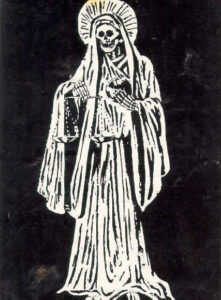
\includegraphics[scale=.5]{a20191027DeathandtheRealI-img001.jpg} 
\caption{Muerte Blanca} 
\end{wrapfigure}

I was driving on the highway at night, paying close attention to the traffic. A cop car ahead of me, a few cars in the lanes to my left. I accidentally turned off my headlights but could not turn them back on. Suddenly, the entire highway was pitch black. I continued to drive, unable to see anything ahead. The brakes did not work, yet the car was accelerating. I was weaving in and out, all the time thinking that I would crash into something. I speculated on what crash would occur while continuing to drive.

The ambiguity was clear. Was I heading into the darkness of death? Or was I being guided by unknown forces?

In Chapter V of \emph{Gnosis} Book 1, Boris Mouravieff includes a meditation on death, which comprised three exercises. The I of the Personality gives little thought to its own death. Mouravieff explains:

\begin{quotex}
All man can imagine in this respect is to evoke the image of his own corpse: he can never exclude from this representation the observer who contemplates this image. 

\end{quotex}

Only the Real I can contemplate one's death. While the ego looks for the light, the Real I faces the darkness. In most cases, it takes a major event, a boundary situations, to get the ego to face its own annihilation. Examples are: fright, guilt, finality, and suffering.

\begin{wrapfigure}{rt}{.3\textwidth}

\includegraphics[scale=.4]{a20191027DeathandtheRealI-img002.jpg} 
\end{wrapfigure}

\paragraph{Exercise 1: Remembrance of death}
\begin{quotex}
Death is the only real and unique event which happens to us without fail. In other words, constantly bearing in mind the idea of death approaching nearer every day is a concrete means of facing an implacable reality — before which all the joys and all the worries of the Personality fade. It is thus that one learns that in effect: `all is vanity and torments of the mind.' 

\end{quotex}
It is insufficient to read this exercise; rather, one must actually do it. The timing is good. During Halloween season in the USA, people decorate their lawns with images of death. Walk around the neighborhood and contemplate the skulls. It is better than candy.

This week: pray for the dead and visit a cemetery.

\paragraph{Exercise 2: The narrow road leading to Life}
\begin{quotex}
This is done by introducing a continuous and permanent attachment between the Personality and the passive Real `I'. so as to render the presence of the latter constant in the field of action of the Personality. Then, with time and according to the intensity of efforts, the situation can undergo a complete change: the more the Real I – like the grain of mustard seed – takes root in the mental life which was until then dominated by the Personality, the more the latter is subjected, little by little, to the will of the judge. Identifying himself with it, man will rediscover his Real `I' in all its integrity and permanence. For him, life then loses its factitious character, to become logical and factual. 

\end{quotex}
Train the ego, or false I, to become aware of the Real I. The ego lies to himself; it sugarcoats his life. The Real I judges rightly, which the ego dislikes. Ultimately, the goal is for the ego to become passive to the Real I. Learn to distinguish between the speech of the ego and the Real I.

\begin{quotex}
When a person speaks, it is generally easy to distinguish whether his records are playing or whether he speaks from some deeper part of himself. In the latter case, he uses a pictorial, rustic and sometimes awkward language; in the former he speaks in a singing tone of voice. 

\end{quotex}
\paragraph{Exercise 3: The philosopher's stone}
\begin{quotex}
The permanent link which must be introduced between the Personality and the real `I' is esoteric Knowledge. The knowledge and know-how that it permits us to acquire represent the philosophers' stone of the medieval mystics. They are capable of provoking in man the transmutation to which he aspires. 

\end{quotex}
Read the best material rather than wild speculations or useless opinions.

\paragraph{Summary:}
\begin{itemize}
\item Constantly bear in mind the idea of your own death 
\item Make the real I the master of the I of the Personality 
\item Acquire esoteric knowledge 
\end{itemize}
\paragraph{Leaving the I of the Personality Behind}
\begin{quotex}
the petty bourgeois is spiritless[.] … Devoid of imagination, as the petty bourgeois always is, he lives within a certain orbit of trivial experiences as to how things come about, what is possible, what usually happens, no matter whether he is a tapster or a prime minister. This is the way the petty bourgeois has lost himself and God. \flright{\textsc{Soren Kierkegaard}, \emph{The Sickness Unto Death}}

\end{quotex}


\flrightit{Posted on 2019-10-27 by Cologero }

\begin{center}* * *\end{center}

\begin{footnotesize}\begin{sffamily}



\texttt{Patricia on 2019-10-28 at 17:05 said: }

Your dream reminds me of the dark night of the senses that St. John of the Cross wrote about. The gift on the other side of that “night” erupts in the last sentence of your writing, concerning the moments when joy and beauty suddenly appear. I am so glad you made it through such a difficult medical and spiritual challenge.


\hfill

\texttt{Santiago on 2020-10-28 at 13:16 said: }

One of my favorite articles on the site. Steps 2 and 3 seem somewhat more difficult!

Regarding step 1, Evola states in Doctrine of Awakening, that it's a good practice to witness an autopsy and meditate on the nature of death. The idea being, if I recall correctly, to maintain an awareness that we are more than our physical body. There are many autopsies one may watch on YouTube, and all are quite grotesque, so squeamish viewers should overlook the provided example: https://www.nsfwyoutube.com/watch?v=nHeFUT-11So (NSFW)

“Only the Real I can contemplate one's death. While the ego looks for the light, the Real I faces the darkness. In most cases, it takes a major event, a boundary situations, to get the ego to face its own annihilation. Examples are: fright, guilt, finality, and suffering.”

Is the sensation of ego annihilation typically accompanied by a `deep' darkness and a profound, rapid sense of `falling'. I had this experience recently, and it was so overwhelming that I impulsively stood up and gasped for air, ending immediately the experience.


\hfill

\texttt{Greg on 2020-10-29 at 14:24 said: }

Is death the annihilation of the personality? If you listen to nde accounts it would seem not but I suppose they might be unreliable.


\end{sffamily}\end{footnotesize}


\chapter{Sparse notes}
\section{Amor Fati and the Heroic Life}

\begin{quotex}
My formula for the greatness of man is amor fati — to change nothing, neither before nor after, throughout all eternity. Not only to bear Necessity, and still less to hide it — all idealism is a lie in the face of Necessity — but to love it. \flright{\textsc{Friedrich Nietzsche}}

A happy life is impossible; the highest to which man can attain is an heroic course of life. \flright{\textsc{Arthur Schopenhauer}}

\end{quotex}
\paragraph{Amor Fati}
The highest form of Amor Fati is to follow the will of God. The first act of will is the acceptance of the circumstances of your birth. To wish it to have been otherwise, is to wish to have been someone else.

When \textbf{Saint Anthony the Great} thought about the depth of the judgments of God, he asked,

\begin{quotex}
Lord, how is it that some die when they are young, while others drag on to extreme old age? Why are there those who are poor and those who are rich? Why do wicked men prosper and why are the just in need? 

\end{quotex}
He heard a voice answering him,

\begin{quotex}
Anthony, keep your attention on yourself; these things are according to the judgment of God, and it is not to your advantage to know anything about them. 

\end{quotex}
\paragraph{The Heroic Life}
To resist the modern world, embrace what is most despised by the modern world and, a fortiori, also despised by some who fantasize about resistance. Embrace the world that valued:

\begin{itemize}
\item Logic, grammar, rhetoric 
\item Geometry, mathematics, music, cosmology 
\item True philosophy in the mould of Plato and Aristotle 
\item Mysticism 
\item Chivalry 
\item Art, Poetry, Architecture 
\item Social Order 
\item Care widows, orphans, the sick, and infirm 
\end{itemize}
Dante showed the path from the bug life (mere animation) to Union with God. The seven stages are described in their all-too-human detail, not as some lifeless abstractions. This path will lead to results and save you years of fruitless seeking. Do not just read, but actually apply, what is contained in these texts:

\begin{itemize}
\item \textbf{Richard of Saint Victor}, \emph{De Contemplatione} 
\item \textbf{Saint Bernard}, \emph{De Consideratione} 
\item \textbf{Saint Augustine}, \emph{De Quantitate Animae} 
\item \textbf{Saint Thomas Aquinas}, \emph{Summa Theologiae} 
\item \textbf{Dante}, \emph{The Divine Comedy} 
\end{itemize}


\flrightit{Posted on 2020-08-07 by Cologero }

\section{Last Word}

The next task is also the last task and therefore the most difficult one. Four things are necessary to fulfil it.

\paragraph{Live by Principles}
Research the principles of \textbf{Bernard of Clairvaux} for a good life and live by them.

That has been your task from the start. Everybody forgot. Do not forget that amongst these principles most important one is to pledge your life and everything that one owns to the cause, defence, honour and further knowledge of the Christian religion and the Holy Church. That means both Catholic and Orthodox Church each with their own dogmas and respective holy centres and patrons. Neither defamation nor furthering of the schism belongs to the life one has been expected to lead. This task also does not have anything to do with common modern day politics and enmities, daily life and journalism, as such are regarded to be realities of a profane nature, so one should relinquish any attempt to conjoin your task with latter. Such is permittable only in one case, that of utmost necessity and solely that — indeed the same you have been called up for — defence, honour and further knowledge of the Christian religion and the Holy Church.

\paragraph{Basic Training}
To be able to live up to these principles, you need to acquire a basic training.

The first steps are: the control of thinking, feeling, willing, control of speech, control of action, all these combined. Not in a 10 minute meditation, not in an exercise, one is also not expected to perfect this as everybody comes to a situation sooner or later where one fails this and shows weakness and doubt. In such situations remember also that Our Lord suffered in Gethsemane, find strength in remembering that nevertheless he completed his Mission in the end for all of us. Try then to accomplish what is asked from this training in situations when it is needed and important.

Correct thought, correct feeling, correct word, correct action.

\paragraph{Mutual Respect}
Observance and Excellence, Education and Culture, Ethics and mutual Respect of other Confessions, as well as always when necessary and possible, mediating a peaceful dialogue between them; furthermore, abiding all written and unwritten laws and mores, national and International — is what is asked from all who decide to follow this path. To achieve these, one should school oneself also in the art of oratory — as a proper expression — so that a man can be considered wise and truthful whether with friends or in the face of adversary, and at both tables he will be respected and well received.

\paragraph{Service}
All these you must not do to excel and take pride in your achievements when you compare yourself with your neighbour. You do all this to serve. Christ washed the feet of his disciples and he was the First among all. Love your neighbour\footnote{Updated 13 IX 2020.

This is the last task assigned to me by a dear spiritual friend. As for the materials sent to me, I have been using them, not always explicitly. Those who are supposed to manage them, can't manage.

But I need to improve German vocabulary so I don't get slowed down looking up words.

As for oratory, I have new audio equipment. But it seems a lot of work for little reach. I'm not Joe Rogan.}.



\flrightit{Posted on 2018-09-13 by Anon }

\begin{center}* * *\end{center}

\begin{footnotesize}\begin{sffamily}



\texttt{Cologero on 2018-09-13 at 22:18 said: }

Very moving, but we have to take into account human capacities. For example, you alluded to some exercises suggested by Rudolf Steiner. As he points out, however, even 10 minutes may be too strenuous for most people. In \emph{Knowledge of Higher Worlds}, he makes this suggestion:

\begin{quotex}
The student must set aside a small part of his daily life in which to concern himself with something quite different from the objects of his daily occupation. The way, also, in which he occupies himself at such a time must differ entirely from the way in which he performs the rest of his daily duties. But this does not mean that what he does in the time thus set apart has no connection with his daily work. On the contrary, he will soon find that just these secluded moments, when sought in the right way, give him full power to perform his daily task[s]. Nor must it be supposed that the observance of this rule will really encroach upon the time needed for the performance of his duties. Should anyone really have no more time at his disposal, five minutes a day will suffice. It all depends on the manner in which these five minutes are spent. 

\end{quotex}

\hfill

\texttt{Anon on 2018-09-14 at 03:19 said: }

When you finish the material I sent you, tell me what you think about then about this same matter. Who cant manage, cant manage. Things are how they are.


\hfill

\texttt{Cologero on 2018-09-14 at 12:22 said: }

Well, Anon, if I have to finish the material first then you have not yet said the Last Word.

The goal is to help serve others (i.e., those who read this blog), as you wrote, not to display one's own superiority.

So let's discuss Steiner's exercise from a book that you recommended to me as part of the “material”. Why do suppose that 5 minutes do not suffice?

The material also includes this passage:

\begin{quotex}
Pay attention to your ideas. Only think important thoughts. Learn to separate in your thoughts the essential from the inessential, the eternal from the transient, the truth from mere opinion.

When listening or talking to one's fellow man, one tries to become completely silent within oneself and to give up all approval, in particular all disparaging judgments, both in thoughts and feelings. 

\end{quotex}
Does that mean we should withhold disparaging judgments, at least until we are sure we understand?

How does one separate the eternal from the transient? Certainly comparing the human condition from 800 years ago to day might be a prelude to that.

When we consider correct speech, the circumstances need to be taken into consideration. What is appropriate in one setting may not be in another. And when is it necessary to speak out? Would it not be correct speech to point out crimes and injustice? Silence is Consent: \textit{Qui tacet consentire videtur, ubi loqui debuit ac potuit}.

You may have forgotten Point 5: forgiveness. Things are not simply how they appear, as you imply. A person does not acquire all those qualities on a balmy weekend. It is the task of a lifetime, and there will be failures on the way, many failures. Forgiveness ought to follow faults, but it seems to be much easier to err than to forgive.


\end{sffamily}\end{footnotesize}



\end{document}
